\chapter{LÝ THUYẾT VỀ CÁC MÔ HÌNH SỬ DỤNG TRONG ĐỀ TÀI}
\section{Lý thuyết mạng nơ-ron}
Neural Network là một mạng lưới gồm nhiều lớp được lấy cảm hứng từ neuron ở não người. Ở đó, lớp đầu tiên để đưa các đặc tính của vật cần dự đoán vào được gọi là Input Layer. Và layer cuối cùng mang kết quả dự đoán gọi Output Layer. Một mạng neuron có thể có hoặc không có các lớp ở giữa Input Layer và Output Layer gọi là Hidden Layer, các Hidden Layer này giúp cho tỉ lệ dự đoán chính xác cao hơn tuy nhiên việc huấn luyện cũng tốn nhiều thời gian và dung lượng hơn. Mỗi Layer là tập hợp nhiều node, các node của lớp sau kết nối với toàn bộ các node của lớp trước.\par
Trong mạng neural network, lớp đầu tiên đưa các đặc tính vào mạng gọi là input layer, lớp cuối cùng để đưa ra các dự đoán gọi là output layer. Giữa $2$ lớp input và output gồm một hoặc nhiều lớp ẩn giúp tăng khả năng học và dự đoán của mạng được gọi là hidden layer. Mỗi layer là tập hợp gồm nhiều node, các node của lớp sau kết nối với \textit{toàn bộ} node của lớp trước.\par
Mỗi node trong hidden layer và output layer thực hiện các công việc sau: Liên kết với tất cả các node ở layer trước đó với các hệ số w riêng. Mỗi node có 1 hệ số bias b riêng. Từ đó w,b biểu thị mối quan hệ giữa node trước và node sau như hình \ref{fig:neural1}.\par
\begin{figure}[ht!]
\centerline{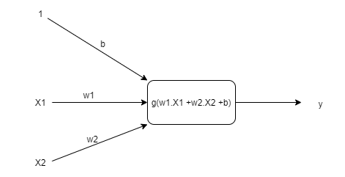
\includegraphics[scale=0.7]{images/neural1.PNG}}
\caption{Mối quan hệ giữa ngõ vào và ngõ ra của một node trong mang nơ-ron.}
\label{fig:neural1}
\end{figure}
Node phía trên có đầu vào là X1,X2, trọng số w1,w2. Ngõ ra y là kết quả của một hàm phi tuyến và một hàm tuyến tính. Hàm phi tuyến còn được gọi là hàm kích hoạt (activation).Các hàm phi tuyến tính (kích hoạt) thường được sử dụng là:\\
\tab \textbf{sigmoid}:Hàm sigmoid có công thức: $sigmoid(z)= \frac{1}{1+e^{-z)}}$ với đồ thị như trong hình \ref{fig:neural2}(a). Nếu đầu vào lớn, hàm số sẽ cho đầu ra gần với 1. Với đầu vào nhỏ (rất âm), hàm số sẽ cho đầu ra gần với 0.\\
\tab \textbf{Tanh}: Giá trị ngõ ra được chuyển về trong khoảng $[-1,1]$ khiến nó có tính chất tâm không (zero-centered)thay vì chỉ dương như sigmoid, có công thức $Tanh(z)=\frac{e^{z}-e^{-z}}{e^z+e^{-z}}$ với đồ thị như hình \ref{fig:neural2}(b).\par
\begin{figure}[ht!]
\centerline{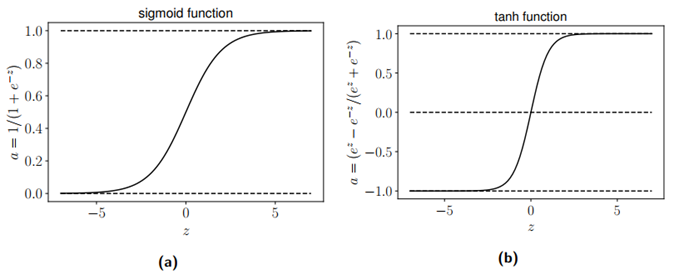
\includegraphics[scale=0.7]{images/neural2.png}}
\caption{Đồ thị hàm sigmoid (a) và hàm tanh (b)\cite{ntt:2019}.}
\label{fig:neural2}
\end{figure}
\noindent\tab\textbf{ReLU và Leaky RELU}: RELU lấy ngưỡng giá trị ở 0 (Thay thế các giá trị âm bằng 0): $RELU(z)= max(0,z)$. Từ đây có thể suy ra chức năng của lớp ReLU là chuyển toàn bộ giá trị âm của ngõ vào (là kết quả lấy từ lớp Convolutional) thành giá trị 0, tạo ra tính phi tuyến cho mô hình để phù hợp với các mẫu trong thực tế không phải lúc nào cũng tuyến tính. Lớp ReLU làm biến đổi ngõ vào và xuất thẳng đến ngõ ra do đó không có trọng số được học trong lớp ReLU \cite{ntt:2019}.
\section{Mang nơ-ron tích chập}
Mạng neural cơ bản khi giải quyết bài toán bài toán xử lý phân loại hình ảnh gặp một số khó khăn. Ví dụ đối với ảnh màu $64*64$ được biểu diễn dưới dạng 1 tensor 3 chiều $64*64*3$. Việc để biểu thị hết nội dung của bức ảnh thì cần truyền vào input layer tất cả các pixel $(64*64*3 = 12288)$. Nghĩa là input layer giờ có 12288 nodes. Giả sử số lượng node trong hidden layer 1 là 1000. Số lượng weight W giữa input layer và hidden layer 1 là $12288*1000 = 12288000$, số lượng bias là 1000 nên tổng số parameter là: 12289000. Đây mới chỉ là số parameter giữa input layer và hidden layer 1, trong model còn nhiều layer nữa, và nếu kích thước cây ảnh tăng, ví dụ $512*512$ thì số lượng parameter tăng cực kì nhanh. Điều này khiến cho việc tính toán của máy tính cần rất nhiều công sức nhưng lại không mang lại hiệu quả cao. \par  
Do vậy ý tưởng sử dụng mạng neural tích chập (Convolutional Neural Network -CNN) ra đời. Áp dụng phép tính convolution vào các layer trong Neural Network ta có thể giải quyết được vấn đề giảm thiểu lượng lớn parameter mà vẫn lấy ra được các đặc trưng của ảnh. Một mô hình mạng CNN sẽ có cấu trúc chung gồm các lớp convolution và các lớp khác như ReLu layer, pooling, fully connected.\par
\subsection{Phép tính tích chập}
Lấy ví dụ trên ảnh xám, ảnh được biểu diễn dưới dạng ma trận A kích thước $m*n$. Ta định nghĩa kernel là một ma trận vuông kích thước $k*k$ trong đó k là số lẻ. k có thể bằng 1, 3, 5, 7, 9,.. Ví dụ kernel kích thước $3*3$. Kí hiệu phép tính convolution là $\otimes$ , kí hiệu $Y = X \otimes W $.\par
Với mỗi phần tử $x_{ij}$ trong ma trận X lấy ra một ma trận có kích thước bằng kích thước của kernel W có phần tử $x_{ij}$ làm trung tâm gọi là ma trận A. Sau đó tính tổng các phần tử của phép tính element-wise của ma trận A và ma trận W, rồi viết vào ma trận kết quả Y. Hình \ref{fig:neural3} mô tả phép tính tích chập $Y = X \otimes W $.\par
\begin{figure}[ht!]
\centerline{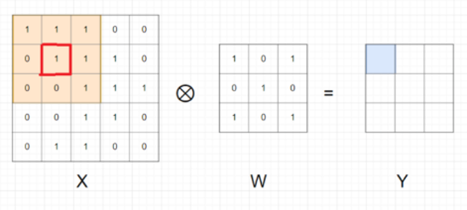
\includegraphics[scale=0.6]{images/neural3.png}}
\caption{Phép tính tích chập $Y = X \otimes W $.}
\label{fig:neural3}
\end{figure}
\subsection{Phép tính Padding và Stride}
\textbf{Padding}: Như ở trên, mỗi lần thực hiện phép tính convolution xong thì kích thước ma trận Y đều nhỏ hơn X. Tuy nhiên giờ ta muốn ma trận Y thu được có kích thước bằng ma trận X, cần hêm giá trị 0 ở viền ngoài ma trận X.\par
\begin{figure}[ht!]
\centerline{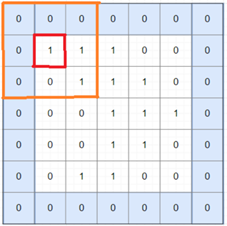
\includegraphics[scale=0.6]{images/neural4.png}}
\caption{Ma trận khi thêm viền 0 bên ngoài.}
\label{fig:neural4}
\end{figure}
Hình \ref{fig:neural4} mô tả một ma trận với padding=1 với những ô vuông màu xanh là những ô vuông được thêm vào ma trận ban đầu. Padding = k nghĩa là thêm k vector 0 vào mỗi phía của ma trận.\par
\textbf{Stride}:Khi thực hiện tuần tự các phần tử trong ma trận X, thu được ma trận Y cùng kích thước ma trận X, ta gọi là $stride = 1$. Tuy nhiên nếu $tride=k (k > 1)s$ thì ta chỉ thực hiện phép tính convolution trên các phần tử $x_{1+i*k,1+j*k}$.\par
\begin{figure}[ht!]
\centerline{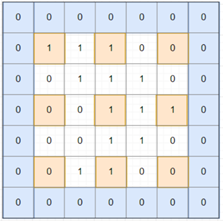
\includegraphics[scale=0.5]{images/neural5.png}}
\caption{Ma trận khi padding = 1, stride = 2.}
\label{fig:neural5}
\end{figure}
Hình \ref{fig:neural5} là ma trận có padding=1. Stride=2. Hiểu đơn giản là bắt đầu từ vị trí $x_{11}$ sau đó nhảy k bước theo chiều dọc và ngang cho đến hết ma trận X. Kích thước của ma trận Y là $3*3$ đã giảm đi đáng kể so với ma trận X. Stride thường dùng để giảm kích thước của ma trận sau phép tính convolution. Công thức tổng quát cho phép tính convolution của ma trận X kích thước m*n với kernel kích thước $k*k$, $stride = s, padding s = p$ ra ma trận Y kích thước :\par
\begin{equation}
\left( \dfrac{m-k+2p}{s}+1\right) *\left( \dfrac{n-k+2p}{s}+1\right) 
\end{equation}
\subsection{Convolutional Layer}
Convolutional Layer là khối xây dựng cốt lõi, nơi thực hiện hầu hết những tính toán nâng cao của một mạng neural tích chập. Một lớp Convolutional Layer gômf một bộ các bộ lọc chứa những tham số có khả năng học và cập nhật theo thời gian. Mỗi bộ lọc là một vùng không gian nhỏ, được đại diện bằng một ma trận số thực. Trong suốt quá trình huấn luyện, bộ lọc này sẽ trượt dọc theo chiều dài và chiều rộng của bức ảnh đầu vào, lần lượt quét 
 những vùng không gian con của bức ảnh và trích xuất đặc trưng trong vùng ấy. Những đặc trưng học đượ được lưu trong ma trận gọi là feature map \cite{ntt:2019}.\par
\begin{figure}[ht!]
\centerline{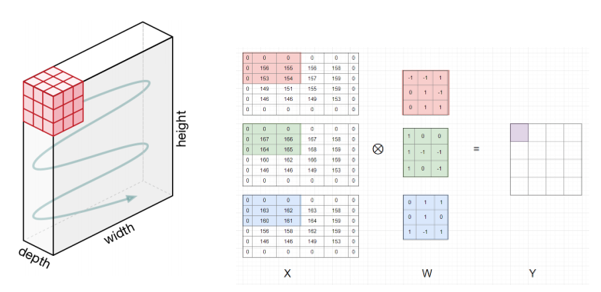
\includegraphics[scale=0.5]{images/neural6.png}}
\caption{Phép tính tích chập trên ảnh màu với filter 3x3 \cite{ntt:2019}.}
\label{fig:neural6}
\end{figure}
Với mỗi kernel khác nhau ta sẽ học được những đặc trưng khác nhau của ảnh, nên trong mỗi convolutional layer ta sẽ dùng nhiều kernel để học được nhiều thuộc tính của ảnh. Vì mỗi kernel cho ra output là 1 matrix nên k kernel sẽ cho ra k output matrix. Ta kết hợp k output matrix này lại thành 1 tensor 3 chiều có chiều sâu k.\par
Output của convolutional layer đầu tiên sẽ thành input của convolutional layer tiếp theo. Convolutional layer tổng quát khi giả sử input của 1 convolutional layer tổng quát là tensor kích thước $H * W * D$.  Kernel có kích thước $F * F * D$ (kernel luôn có depth bằng depth của input và F là số lẻ), stride: S, padding: P. Convolutional layer áp dụng K kernel. Output của layer là tensor 3 chiều có kích thước: \par
\begin{equation}
\left(\dfrac{H-F+2P}{S}+1\right)*\left(\dfrac{H-F+2P}{S}+1\right)* K
\end{equation}
\subsection{Pooling Layer}
Lớp pooling thường được sử dụng ngay sau lớp convulational để đơn giản hóa thông tin đầu ra để giảm bớt số lượng neuron. Mục đích của pooling rất đơn giản, nó làm giảm số hyperparameter mà ta cần phải tính toán, từ đó giảm thời gian tính toán, tránh overfitting. Có 2 loại pooling layer phổ biến là: max pooling và average pooling.\par
\begin{figure}[ht!]
\centerline{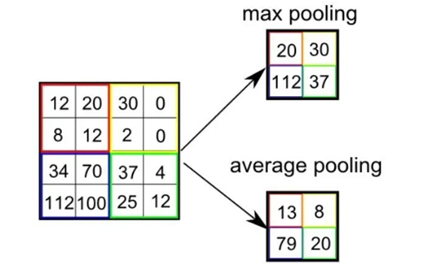
\includegraphics[scale=0.7]{images/neural7.png}}
\caption{Ví dụ về Pooling Layer \cite{ntt:2019}}
\label{fig:neural7}
\end{figure}
\subsection{Fully Connected Layer}
Sau khi ảnh được truyền qua nhiều convolutional layer và pooling layer thì model đã học được tương đối các đặc điểm của ảnh (ví dụ mắt, mũi, khung mặt,…) thì tensor của output của layer cuối cùng, kích thước $H*W*D$, sẽ được chuyển về 1 vector kích thước $(H*W*D)$. Sau đó ta dùng các fully connected layer để kết hợp các đặc điểm của ảnh để ra được output của model \cite{ntt:2019}.\par
\begin{figure}[ht!]
\centerline{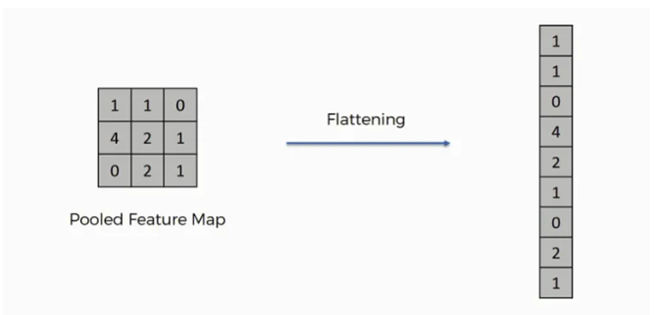
\includegraphics[scale=0.7]{images/neural8.png}}
\caption{Hình phép Flatten biến đổi tensor về 1 vector \cite{ntt:2019}.}
\label{fig:neural8}
\end{figure}

\section{Mạng Mobilenet}
Ở mô hình mạng MobileNet v1, ta sử dụng các lớp tích chập depthwise Seperable, một tích chập tối ưu hơn so với tích chập thông thường như đã trình bày ở phần 2.2. Ở mô hinh này, lớp tích chập depthwise sử dụng những filter đơn lẻ cho từng kênh ngõ vào (input channel). Lớp tích chập pointwise sử dụng tích chập 1x1 để kết hợp các ngõ ra của lớp tích chập depthwise. Lớp tích chập thông thường thực hiện cả việc lọc và kết hợp input trong một lần. Lớp tích chập depthwise separable chia nó ra làm 2 giai đoan, một giai đoạn riêng cho việc lọc và một giai đoạn riêng cho việc kết hợp. Điều này đã giúp mang lại hiệu quả lớn trong việc giảm số lượng tính toán và kích thước mô hình \cite{mobile:viblo}.\par

Giả sử ảnh đầu vào có kích thước $12*12*3$, thực hiện 1 phép tích chập có cửa số $5*5$ lên ảnh đó với $padding = 0$ và $stride = 1$ như hình \ref{fig:mobi1}. Nếu chỉ xét trên chiều dài và rộng của ảnh thì quá trình chập là $(12*12)\rightarrow(5*5) \rightarrow (8*8)$. Cửa sổ lướt qua toàn bộ ảnh, mối lần thực hiện 25 phép nhân và trả về 1 điểm ảnh. Vì $padding =0$ nên ngõ ra là $(8*8)$. Tuy nhiên, ảnh đầu vào có 3 chiều, do đó thay vì thực hiện 25 phép nhân, ta phải thực hiện 75 phép nhân cho mỗi lần kernel dịch chuyển. Giả sử ta sử dụng 256 kernel, vậy ngõ ra sẽ là $8*8*256$. Để tạo ra được ngõ ra này, ta phải thực hiện $256*5*5*8*8*3= 1,228,800$ phép nhân. Đây là một con số vô cùng lớn, do đó mạng nơ ron thông thường không thể sử dụng trong các mô hình nhúng \cite{mobile:viblo}.\par
\begin{figure}[ht!]
\centerline{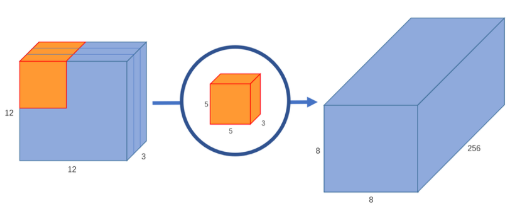
\includegraphics[scale=0.9]{images/mobi1.png}}
\caption{Thực hiện tích chập thông thường \cite{mobile:viblo}.}
\label{fig:mobi1}
\end{figure}
Thực hiện phép chập depthwise seperable tức là thực hiện lần lượt phép chập depthwise và phép chập pointwise. Ta thực hiện phép chập depthwise seperable với cùng ví dụ trên với ảnh đầu vào $12*12*3$. Đầu tiên, thực hiện chập depthwise bằng cách sử dụng 3 kernel $5*5*1$. Ở đây, mỗi kernel sẽ thực hiện phép chập với mỗi channel của ảnh đầu vào, cho ra output $8*8*1$, gộp các kết quả lại, ta thu được ảnh đầu ra $8*8*3$ như hình \ref{fig:mobi2}.\par

\begin{figure}[ht!]
\centerline{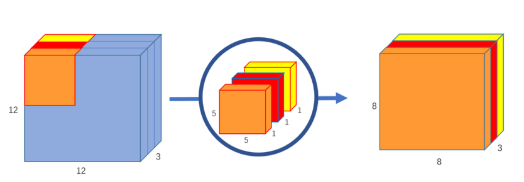
\includegraphics[scale=0.9]{images/mobi2.png}}
\caption{Thực hiện tích chập depthwise \cite{mobile:viblo}.}
\label{fig:mobi2}
\end{figure}
Để thu được ngõ ra có chiều là $8*8*256$, tiếp theo cần tăng số lượng channel lên 256. Đây là nhiệm vụ của tích chập pointwise. Tích chập này sử dụng các kernel có kích thước là $1*1$ để thực hiện phép chập ở từng điểm dữ liệu, số lượng kernel bằng với số lượng channel của ảnh đâu vào với mục đích thu được 1 channel của ảnh đầu ra. Ở ví dụ này, kernel sẽ là $1*1*3$, out put sẽ là $8*8*1$ như hình \ref{fig:mobi3}.\par
\begin{figure}[ht!]
\centerline{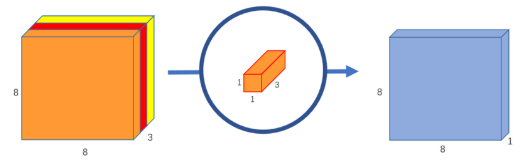
\includegraphics[scale=0.9]{images/mobi3.png}}
\caption{Thực hiện tích chập pointwise,biến đổi ảnh thành 1 channel \cite{mobile:viblo}.}
\label{fig:mobi3}
\end{figure}
Sau đó, sử dụng 256 kernel $1*1*3$ ta được ảnh đầu ra là $8*8*256$ như hình \ref{fig:mobi4}.\par
\begin{figure}[ht!]
\centerline{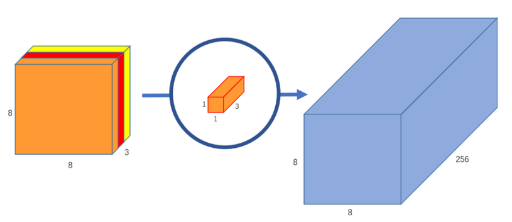
\includegraphics[scale=0.9]{images/mobi4.png}}
\caption{Sử dụng tích chập pointwise với 256 kernels, ngõ ra là ảnh với 256 kernel \cite{mobile:viblo}.}
\label{fig:mobi4}
\end{figure}
Như vậy, sau khi thực hiện 2 phép chập với cùng một ngõ vào và ngõ ra, ta so sánh số phép nhân cần thực hiện để thấy được đặc điểm nổi bật của tích chập depthwise separable so với tích chập thông thường. Đối với tích chập thông thường, thực hiện chập 256 kernel $5*5*3$ trên $8*8$ điểm của ảnh đầu vào, nghĩa là thực hiện $256*3*5*5*8*8 = 1,228,800$ phép nhân. Đối với tích chập depthwise separable, khi thực hiện phép chập depthwise, sử dụng 3 kernels $5*5*1$, kernel dịch chuyển $8*8$ lần, nghĩa là thực hiện $3*5*5*8*8 = 4,800$ phép nhân. Khi thực hiện chập pointwise, chúng ta có 256 kernel $1*1*3$ dịch chuyển $8*8$ lần, tức là $256*1*1*3*8*8= 49,152$ phép nhân. Tổng cộng cả 2 giai đoạn là $53,952$ phép nhân. Số $53,953$ nhỏ hơn $1,228,800$ rất nhiều, do đó mô hình mạng sẽ nhẹ hơn và khả năng thực hiện nhanh hơn rất nhiều lần so với các phép nhân convolution thông thường.

\section{Mạng EfficientNet}
%\cite{efficientnet:2020}
\subsection{Giới thiệu mạng EfficientNet}
Convolutional Neural Networks (ConvNets) thường được hiệu chỉnh một số thông số trong mô hình để tối ưu về độ chính xác và số lượng thông số. Các thông số liên quan đến cấu trúc mạng baseline được hiệu chỉnh gồm độ sâu(depth), độ rộng(width) và độ phân giải(image resolution). Trong mô hình ResNet, tác giả đã điều chỉnh số lượng Layer tạo ra các mô hình như ResNet-18,ResNet-200. Trong mô hình GPipe, tác giả tăng độ lớn của baseline lên 4 lần để đạt được độ chính xác cao hơn. Tuy nhiên, các mô hình này thường điểu chỉnh một trong 3 thông số (depth, width, resolution). Ở mô hình EfficientNet, tác giả thay đổi đông thời cả 3 thông số này một cách có hệ thống dựa theo phương pháp \textit{Compound coefficient}.\par 
Mô hình EfficientNet B7 hiện tại đã đạt "state-of-art" đối với tập ảnh ImageNet khi đạt Top1 accuracy là $84.3\%$ và đối với tập CIFAR-100 là $91.7\%$. Độ chính xác và số lượng thông số của mạng EfficientNet so với các mạng ConvNet khác được thể hiện trên hình \ref{fig:eff1}.\par
\begin{figure}[ht!]
\centerline{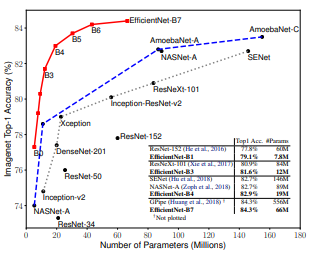
\includegraphics[scale=0.8]{images/eff1.png}}
\caption{So sánh các mô hình trên tập ImageNet \cite{efficientnet:2020}.}
\label{fig:eff1}
\end{figure}
Khi tiếp cận bài toán dự đoán bệnh xơ phổi của bệnh nhân, nhóm quan tâm đến độ chính xác mô hình hơn so với tốc độ xử lý. Vì vậy trong số các mô hình, nhóm nhận thấy EfficientNet (mạng back-bone - trích xuất dữ liệu) của EfficientDet tuy tốc độ xử lí thấp khó đáp ứng realtime nhưng độ chính xác cao nên quyết định sử dụng mạng Efficient Net để dự đoán.\par
\subsection{Thu phóng mô hình}
Để thay đổi một mô hình sao cho có độ chính xác và tốc độ xử lý cao hơn, các mạng thường tiếp cận theo 4 hướng chính: Thay đổi chiều sâu của mạng, thay đổi chiều rộng của mạng, thay đổi độ phân giải đầu vào và thay đổi cấu trúc của từng lớp. Tuy nhiên mục tiêu mà Efficient Net tiếp cận là sử dụng những mạng cơ bản đơn giản như MobileNet và không thay đổi cấu trúc của mạng này, chỉ thay đổi đồng thời chiều sâu, chiều rộng của mạng cũng như độ phân giải của đầu vào sao cho đạt độ chính xác cao. Điều này được gọi là Model Scaling (thu phóng mô hình).\par
\begin{figure}[ht!]
\centerline{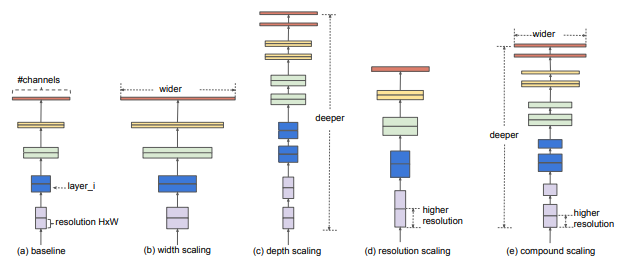
\includegraphics[scale=0.7]{images/eff2.png}}
\caption{ Cách thu phóng mô hình (a) Mô hình gốc (b) Mô hình thu phóng theo chiều rộng (c) Mô hình thu phóng theo chiều sâu
(d) Mô hình thu phóng theo độ phân giải
(e) Mô hình thu phóng kết hợp 3 loại thu phóng theo chiều sâu, rộng và độ phân giải
\cite{efficientnet:2020}.}
\label{fig:eff2}
\end{figure}
Thu phóng theo chiều sâu được thực hiện bằng cách thêm hoặc bớt một số lớp cho mô hình. Việc thu phóng mô hình theo chiều sâu nếu hợp lý có thể trích xuất được các đặc trưng phức tạp và phong phú hơn. Thu phóng theo chiều rộng tức là thêm dữ liệu đầu vào và thêm các node cho từng lớp. Việc thu phóng mô hình theo chiều rộng cũng cần hợp lý, nếu đủ rộng các đặc trưng được trích xuất một cách chi tiết hơn. Thu phóng theo độ phân giải là việc tăng giảm độ phân giải cho dữ liệu ảnh đầu vào để bức hình có thêm nhiều đặc trưng hơn. Thu phóng độ phân giải một cách hợp lý cũng giúp cho mô hình thu được nhiều đặc trưng có chi tiết nhỏ mà có thể bị bỏ sót nếu không thu phóng độ phân giải. Tuy nhiên nếu 3 việc thu phóng này diễn ra một cách không hợp lý, tăng quá sâu hay quá rộng mô hình, tăng độ phân giải lên quá cao sẽ dễ dẫn tới overfitting hay vanishing gradient do học được quá nhiều đặc trưng mang tính cá biệt.\par
Như vậy, tác giả gọi $Y_i=\mathcal{F}_i(X_i)$  trong đó Yi là tensor ngõ ra của lớp thứ i, Xi là tensor ngõ vào của lớp thứ i và Fi là toán tử được thực hiện ở lớp thứ i. Vậy với một mạng có k lớp, mạng đó được định nghĩa công thức \eqref{equa:eff1}:
\begin{equation}
\mathcal{N}= \mathcal{F}_k \odot \mathcal{F}_{k-1}\odot... \odot \mathcal{F}_1=\odot_{j=1..k} \mathcal{F}_j(X_1) \label{equa:eff1}
\end{equation}
Nhiều lớp có cấu trúc giống nhau thường được gom lại thành 1 tầng ( 1 stage ). Khi đó công thức \eqref{equa:eff1} được viết lại như công thức \eqref{equa:eff2}.
\begin{equation}
\mathcal{N}= \odot_{i=1...s} \mathcal{F}^{L_i}_iX_{<H_i,W_i,C_i>} \label{equa:eff2}
\end{equation}
Trong đó i là chỉ số tầng, $H_i,W_i,C_i$ lần lượt là chiều dài, chiều rộng và chiều sâu của đầu vào X.Hàm mục tiêu của EfficientNet là $$Max Accuracy(\odot_{i=1..s} \hat{F}_i^{d.\hat{L}_i} X_{<r.\hat{H}_i,r.\hat{W}_i,w.\hat{C}_i>}$$ Trong đó r,w,d là thông số hiệu chỉnh mạng, $\hat{F}_i,\hat{L}_i,\hat{W}_i,\hat{H}_i,\hat{C}_i$ là thông số của mạng baseline trước khi hiệu chỉnh.\par
\subsection{Thu phóng kết hợp}
Nhóm tác giả thực hiện thu phóng trên tập ImageNet với các kích thước khác nhau và nhận thấy rằng các chiều của mô hình không thu phóng độc lập với nhau. Nếu thực hiện thu phóng độc lập như hình \ref{fig:eff3}, độ chính xác của mạng ban đầu tăng nhanh nhưng sau đó trở nên bão hòa và không thay đổi. Nhưng nếu thực hiện thu phóng kết hợp, độ chính xác của mô hình tăng rõ rệt như hình \ref{fig:eff4}.\par
\begin{figure}[ht!]
\centerline{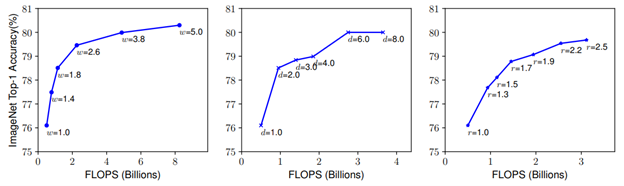
\includegraphics[scale=0.7]{images/eff3.png}}
\caption{Thu phóng lần lượt theo độ rộng, độ sâu và độ phân giải, ta thấy với ban đầu FLOPS (tốc độ tính số floating point trên giây) và độ chính xác ban đầu tăng rõ rệt nhưng càng về sau càng bão hòa\cite{efficientnet:2020}.}
\label{fig:eff3}
\end{figure}

\begin{figure}[ht!]
\centerline{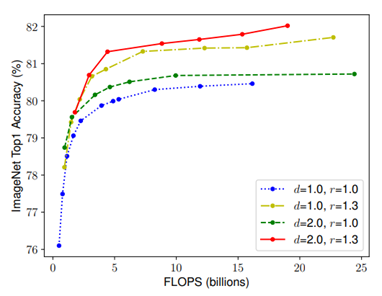
\includegraphics[scale=0.7]{images/eff4.png}}
\caption{Thực hiện thu phóng đồng thời cả chiều rộng và chiều sâu (màu đỏ) cho kết quả cải thiện \cite{efficientnet:2020}.}
\label{fig:eff4}
\end{figure}
Từ đó tác giả đề cập đến một hệ số $\phi$ là mối liên hệ giữa chiều dài, chiều rộng và chiều sâu:\par

$$d=\alpha^\phi$$ 
$$w= \beta^\phi $$
$$r= \gamma^\phi$$ 
$$\alpha.\beta^2.\gamma^2 \approx 2$$ 
$$\alpha\geq1, \beta\geq1,\gamma\geq1$$
Trong đó $\phi$ là hệ số do có thể chỉ định để kiểm soát chiều dài, chiều sâu và độ phân giải của mô hình, $\alpha,\beta,\gamma$ là chỉ cách gán cho chiều dài, chiều sâu và độ phân giải. Kèm theo đó tác giả cũng có ràng buộc  . Hệ số FLOPS tỉ lệ thuận với chiều sâu, bình phương chiều rộng và bình phương độ phân giải. Vì vậy tác giả ràng buộc để FLOPS sẽ tăng theo tỉ lệ $2^\phi$
\subsection{EfficientNet B0 - EfficientNet B7}
Tương tự mạng MnasNet, tác giả cũng sử dụng hàm tối ưu mục tiêu cho mô hình là:\par
$$ACC(m)*\left[ \dfrac{FLOPS(m)}{T}\right]^w$$\par
Trong đó T là mức FLOPS mục tiêu, $ACC(m)$ và $FLOPS(m)$ là độ chính xác và FLOPS mục tiêu của mô hình m, $w = -0.07$ là siêu tham số để kiểm soát sự cân bằng giữa ACC và FLOPS. Mục tiêu FLOPS của EfficientNet là vào khoảng 400M.Đầu tiên, tác giả sử dụng mô hình Efficient Net B0 đơn giản như hình \ref{fig:eff5}:\par
\begin{figure}[ht!]
\centerline{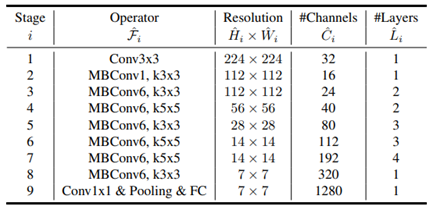
\includegraphics[scale=0.6]{images/eff5.png}}
\caption{Mô hình Efficient Net B0\cite{efficientnet:2020}.}
\label{fig:eff5}
\end{figure}
Trong đó MBConv là mô hình Mobile Convolution Network. Từ mô hình Base 0 này, đầu tiên tác giả giữ nguyên giá trị $\phi=1$. Rồi áp dụng gmall grid tìm kiếm và ràng buộc $\alpha.\beta^2.\gamma^2\approx 2$ để tính ra 3 giá trị còn lại $\alpha=1.2, \beta=1.1, \gamma=1.15$. Tiếp tục, giữ cố định $\alpha,\beta,\gamma$ rồi thu phóng mạng với $\phi$ khác nhau để thu được các EfficientNet từ B0 đến B7. Kết quả thực nghiệm so sánh trên hình \ref{fig:eff6} cho thấy kết quả tốt hơn so với các mô hình trước.
\begin{figure}[ht!]
\centerline{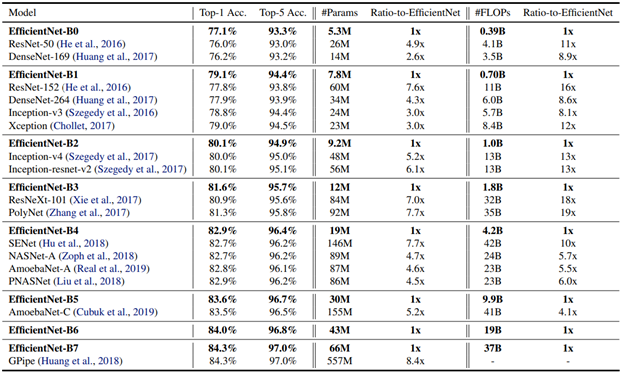
\includegraphics[scale=0.6]{images/eff6.png}}
\caption{So sánh độ chính xác top-1 (kết quả có dự đoán cao nhất trùng với kết quả), độ chính xác top-5(trong 5 kết quả dự đoán cao nhất có kết quả), số tham số,FLOPS \cite{efficientnet:2020}.}
\label{fig:eff6}
\end{figure}
\section{Mô hình Linear Regression}
Regression là phương pháp nghiên cứu mối quan hệ giữa 2 biến mà cụ thể một biến sẽ là biến độc lập, biến còn lại sẽ là biến mục tiêu (bị ảnh hưởng bởi biến độc lập) , mô hình hóa, định lượng hóa mối quan hệ này để qua đó có thể xác định được giá trị của biến mục tiêu nếu các biến độc lập thay đổi như thế nào.\par
Linear regression là mô hình nghiên cứu mối quan hệ tuyến tính giữa một số biến độc lập và biến phụ thuộc. Phương trình tổng quát là 
$$y \approx f(x) = \hat{y}$$
$$f(x) = w_1x_1+w_2x_2+ w_3x_3+w0$$
Với $w_1,w_2,w_3, w_0$ là các hằng số. Bài toán đi tìm các hệ số tối ưu ${w_1,w_2,w_3, w_0}$.\par
Đặt $\textbf{w}= [w_0,w_1,w_2,w_3]^T$ là vector cột cần phải tối ưu và $\overline{\textbf{x}}=[1,x_1,x_2,x_3]$ là vector hàng dữ liệu đầu vào mở rộng, khi đó, phương trình tôngr quát được viết lại là :$$y \approx \overline{\textbf{x}}\textbf{w}  = \hat{y}$$
Hàm mất mát của bài toán Linear Regression là 
$$ \mathcal{L}(\textbf{w}=\dfrac{1}{2}\sum_{i=1}^{N}(y_i-\overline{\textbf{x}}\textbf{w})^2$$
Trong lúc huấn luyện, ta mong muốn sự mất mát nhỏ nhất, ta đạo hàm theo \textbf{w} của hàm mất mát:
$$\dfrac{\partial \mathcal{L}}{\partial \textbf{w}}= \overline{\textbf{X}}^T(\overline{\textbf{X}}\textbf{w}-\textbf{y})$$
Vớí khái niệm giả nghịch đảo, điểm tối ưu của bài toán Linear Regression có dạng:

$$\textbf{w} = \textbf{A}\dagger \textbf{b} = (\overline{\textbf{X}}^T )\overline{\textbf{X}} \dagger \overline{\textbf{X}}^T \textbf{y}$$ 

Quantile Regression là mô hình hổi quy mở rộng của hồi quy tuyến tính - Linear regression, tìm hiểu mối quan hệ tuyến tính giữa biến độc lập và biến phụ thuộc trong trường hợp bộ dữ liệu có các giá trị ngoại lệ (outliers), độ lệch/ chiều cao của phân phối dữ liệu (high skewness), mức độ không đồng nhất của dữ liệu.\par
Mô hình dựa trên xem xét phân phối tổng thể của dữ liệu, không chỉ sử dụng mỗi giá trị trung bình để tính toán, xây dựng công thức như linear regression.\par

Quantile hay còn gọi là phân vị trong thống kê, là phương pháp xác định với $n\%$ bất kì của bộ dữ liệu thì phân phối các giá trị của dữ liệu trong $n\%$ là như thế nào (như các giá trị đã được sắp xếp từ nhỏ tới lớn) để đánh giá độ phân tán của dữ liệu, và tại phân vị thứ n này giá trị của biến là bao nhiêu.\par

\begin{equation}
y = \beta'X_i +\varepsilon_i
\end{equation}
Công thức tính sai số có trọng số theo mô hình hồi quy:\par
\begin{equation}
\tau \sum_{y_i>\hat{\beta}_{\tau}'X_i}\vert y_i- \hat{\beta}_\tau'X_i\vert + (1-\tau)\sum_{y_i<\hat{\beta}_{\tau}'X_i}\vert y_i- \hat{\beta}_\tau'X_i\vert
\label{equa:quan1}
\end{equation}

Phương trình tổng quát của Quantile Regression tương tự như Linear regression, tuy nhiên Quantile Regression hướng đến giảm thiểu sai số của mô hình với phương trình như phương trình \eqref{equa:quan1} .